% !TEX root = ../main.tex
\chapter{Money, Banking, and Monetary Policy}
\label{ch:money}

Almost everything in macroeconomics that we have studied so far --- output, capital, labor, growth --- could in principle be described without ever mentioning money. The Solow and neoclassical models of Chapters~\ref{ch:solow} and~\ref{ch:neoclassical} are written entirely in terms of real goods. Yet no modern economy operates without money, and a great deal of what a government actually \emph{does} to manage the macroeconomy in the short run is done through the central bank. This chapter is about the plumbing: what money is, how the banking system manufactures most of it, and the instruments a central bank uses to expand or contract the supply of credit.

The subject is unavoidably more institutional than the models that came before. Where there is a clean structure --- the liquidity ordering of assets, the money multiplier, the central-bank balance sheet --- we will state it precisely. But much of monetary policy is a matter of who does what to whom through which legal instrument, and these arrangements differ sharply across countries. The two reference systems throughout are the United States, where the central bank operates mostly through the Treasury bond market, and China, where the central bank operates mostly through the commercial banks directly. We treat the China-specific machinery in some detail, because the lecture does, and because it is the cleaner illustration of how a central bank steers an economy through the banking channel. Unless stated otherwise, ``the central bank'' below means the People's Bank of China (PBoC).

Two topics that might seem to belong here have been placed elsewhere. The consumer and producer price indices (CPI and PPI), our measures of the price level, were developed in Chapter~\ref{ch:prices}. The quantity theory of money, the inflation tax, and seigniorage --- the consequences of \emph{printing} money rather than the mechanics of \emph{managing} it --- are the subject of Chapter~\ref{ch:quantity}. Here we stay with the institutions.

\section{Money and Liquidity}

Money is best understood as an \emph{asset} --- a thing of value that one can hold --- distinguished from other assets by one property above all: liquidity. An asset is liquid to the extent that it can be exchanged for goods quickly, cheaply, and at a predictable value. Cash in hand is the limiting case: it is accepted everywhere, instantly, at face value. A government bond, a mutual-fund share, or a publicly traded stock is also a store of value, but converting it into spendable purchasing power takes time and may force a sale at an unfavorable price. The defining feature of money is that it sits at the high-liquidity end of this spectrum.

What makes an asset acceptable as money is ultimately \emph{credibility}: people take it in exchange only because they are confident others will take it from them in turn. The wider that acceptance, the more liquid the asset. Figure~\ref{fig:macro-10} arranges the major financial assets along this dimension.

\begin{figure}[h]
\centering
\begin{tikzpicture}[font=\small]
  % --- geometry of the spectrum ---
  \def\W{14.0}        % total width of the arrow body
  \def\H{1.4}         % half-height of the arrow body
  \def\head{1.6}      % horizontal length of the arrowhead
  \def\tip{2.05}      % half-height at the base of the arrowhead

  % wide right-pointing arrow (least liquid on the left, most liquid on the right)
  \draw[line width=0.8pt, rounded corners=2pt, fill=black!6]
        (0,\H) -- (\W,\H) -- (\W,\tip)
        -- (\W+\head,0)
        -- (\W,-\tip) -- (\W,-\H) -- (0,-\H) -- cycle;

  % --- four rounded boxes inside the arrow, left to right ---
  \tikzset{libox/.style={draw, line width=0.8pt, rounded corners=5pt,
                         minimum height=1.55cm, align=center,
                         inner sep=4pt, anchor=center}}

  \node[libox, minimum width=2.95cm] (b1) at (1.85,0)
        {Government bonds,\\ funds, stocks};
  \node[libox, minimum width=2.45cm] (b2) at (5.35,0)
        {Time deposits};
  \node[libox, minimum width=4.0cm] (b3) at (9.3,0)
        {Checks,\\ demand deposits};
  \node[libox, minimum width=1.75cm] (b4) at (12.85,0)
        {Cash};

  % --- caption beneath: increasing liquidity ---
  \draw[-Latex, line width=0.9pt] (0,-2.55) -- (\W+\head,-2.55);
  \node[below, anchor=north] at ({(\W+\head)/2},-2.62) {increasing liquidity};
\end{tikzpicture}

\caption{The liquidity spectrum, from the least-liquid assets (bonds, fund shares, stocks) on the left to the most-liquid asset, cash, on the right.}
\label{fig:macro-10}
\end{figure}

\defn{Liquidity}{
The \emph{liquidity} of an asset is the ease with which it can be converted into a generally accepted means of payment without loss of value. Money is, by definition, the most liquid class of assets; cash is the most liquid form of money.
}

A useful corollary is that liquidity is priced. A less liquid asset must offer a \emph{premium} --- a higher expected return or a discount in price --- to be held alongside more liquid ones; otherwise no one would accept the inconvenience of holding it. This single idea, that low-liquidity assets trade at a discount to high-liquidity ones, organizes much of what the banking system and the central bank do.

\begin{remark}[Banking as a liquidity transformation]
A bank loan is collateralized: the borrower pledges a low-liquidity asset (a house, a bond, a factory) and receives high-liquidity funds in return. The borrower's illiquid wealth is, in effect, swapped for liquid purchasing power, and the \emph{total} liquidity available to the real economy rises even though no new real asset has been created. The central bank does exactly the same thing one level up: it lends to commercial banks against collateral such as government bonds, swapping the banks' less-liquid holdings for the most-liquid asset of all. Managing the economy's liquidity is the central bank's day-to-day business. When the Treasury collects taxes, for instance, it drains liquidity out of the private sector; the central bank typically offsets this by injecting base money, so that the tax round does not cause an unintended monetary contraction.
\end{remark}

\section{Monetary Aggregates}

Because ``money'' covers assets of differing liquidity, statistical agencies do not report a single number for it. They report a nested family of \emph{monetary aggregates}, each adding a layer of less-liquid, more deposit-like instruments to the one inside it. Figure~\ref{fig:macro-11} shows the standard nesting, $M_0 \subset M_1 \subset M_2$.

\begin{figure}[h]
\centering
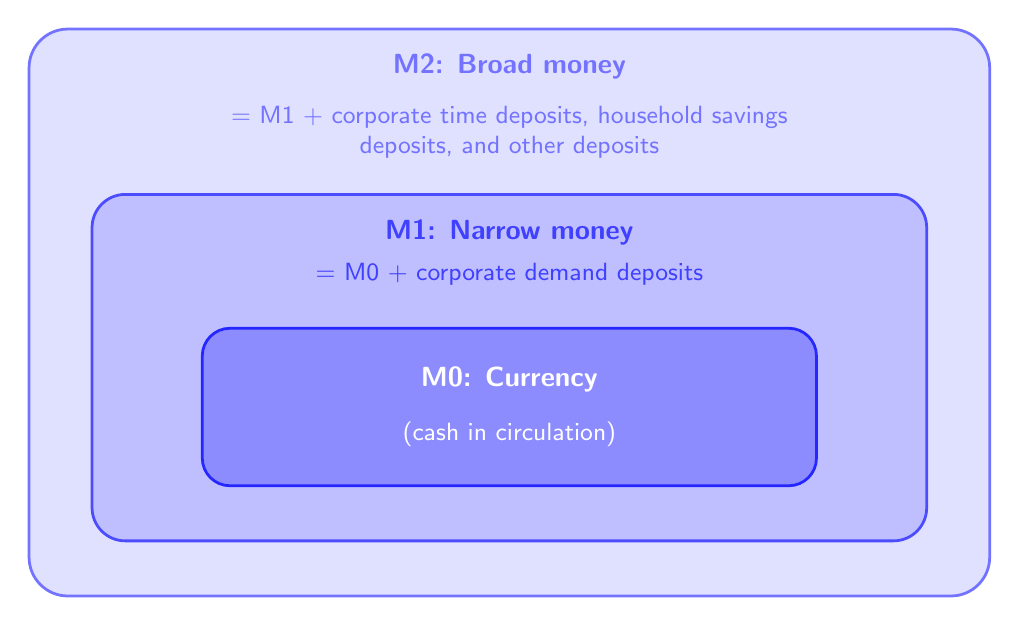
\begin{tikzpicture}[font=\sffamily]
  % Monetary aggregates as TRUE nested containment: M2 contains M1 contains M0.
  % Graduated blue shades convey the subset relation M2 \supset M1 \supset M0:
  % outermost lightest (M2), middle (M1), innermost darkest (M0).

  % --- M2: outer, lightest box (broad money) ---
  \draw[fill=blue!12, draw=blue!55, line width=1pt, rounded corners=14pt]
    (0,0) rectangle (12.2,7.2);
  \node[anchor=north, font=\sffamily\bfseries, text=blue!55] at (6.1,7.0)
    {M2: Broad money};
  \node[anchor=north, align=center, text width=11.6cm, font=\sffamily\small,
        text=blue!55] at (6.1,6.35)
    {$=$ M1 $+$ corporate time deposits, household savings\\
     deposits, and other deposits};

  % --- M1: middle box, lighter shade (narrow money) ---
  \draw[fill=blue!25, draw=blue!70, line width=1pt, rounded corners=12pt]
    (0.8,0.7) rectangle (11.4,5.1);
  \node[anchor=north, font=\sffamily\bfseries, text=blue!75] at (6.1,4.9)
    {M1: Narrow money};
  \node[anchor=north, align=center, text width=9.8cm, font=\sffamily\small,
        text=blue!75] at (6.1,4.35)
    {$=$ M0 $+$ corporate demand deposits};

  % --- M0: inner box, darkest shade (currency) ---
  \draw[fill=blue!45, draw=blue!85, line width=1pt, rounded corners=10pt]
    (2.2,1.4) rectangle (10.0,3.4);
  \node[font=\sffamily\bfseries, text=white] at (6.1,2.75)
    {M0: Currency};
  \node[align=center, text width=7.0cm, font=\sffamily\small, text=white]
    at (6.1,2.05)
    {(cash in circulation)};
\end{tikzpicture}

\caption{The nested monetary aggregates: currency $M_0$ sits inside narrow money $M_1$, which sits inside broad money $M_2$.}
\label{fig:macro-11}
\end{figure}

\defn{Monetary Aggregates}{
The monetary aggregates order money by liquidity:
\begin{itemize}
    \item $M_0$ --- currency in circulation: physical cash held outside the banking system, the most liquid component.
    \item $M_1$ --- ``narrow money'': $M_0$ plus demand (checkable) deposits, which can be spent on short notice.
    \item $M_2$ --- ``broad money'': $M_1$ plus time and savings deposits, which are slightly less liquid.
\end{itemize}
Each aggregate strictly contains the ones inside it.
}

The cash component $M_0$ is small and is driven mainly by short-run, seasonal factors (holidays, payroll cycles). The aggregate that matters for policy is $M_2$. Cash is only a tiny fraction of $M_2$; the overwhelming bulk of ``money'' in a modern economy is not paper at all but \emph{deposit balances} --- entries on banks' books. In a slogan: money is the figure on the ledger.

\begin{remark}[Money held versus money in society]
$M_0$, $M_1$, and $M_2$ all measure money that the public actually holds. This is not the same as the total quantity of money the system could create, nor the same as ``wealth.'' The aggregates are stocks of liquid claims in circulation at a point in time, no more and no less; do not read them as a census of all purchasing power in the economy.
\end{remark}

\subsection{Why \texorpdfstring{$M_2$}{M2} is the policy target}

$M_2$ is the lens through which monetary growth is viewed. The \emph{growth rate} of $M_2$ is the headline measure of monetary policy; in China a target of roughly ten percent has often been set at the annual ``Two Sessions.'' As a rule of thumb, the growth of $M_2$ is expected to roughly track the growth of nominal GDP --- enough new money to finance the new transactions, no more. Strictly, though, this rule cannot hold mechanically, because the whole point of monetary policy is \emph{countercyclical}: the central bank deliberately lets money grow faster than output in a downturn and slower in a boom. A money supply that simply matched nominal GDP every quarter would be doing no stabilizing work at all.

\begin{remark}[The $M_2/\mathrm{GDP}$ ratio is easy to misread]
China's ratio of $M_2$ to GDP exceeds 200\%, while the United States' is under 100\%. It is tempting to conclude that China is awash in excess liquidity and the U.S.\ is not. The comparison does not support that conclusion, for several reasons.

First, the two central banks behave very differently: the PBoC has historically been restrained in expanding the money supply, whereas the Fed swings aggressively (sharp cuts in crises, later reversals). Second, and more fundamentally, the \emph{channel} through which $M_2$ is created differs. In common-law economies such as the U.S.\ and U.K., \emph{direct finance} dominates: firms raise money chiefly by issuing bonds and stocks, which do not pass through and inflate bank-deposit aggregates. China relies on \emph{indirect finance}: firms borrow from commercial banks, and every such loan creates a matching deposit, so a credit-driven economy mechanically carries a larger $M_2$ relative to GDP. The commercial banks are the central hub of the Chinese financial system. Third, $M_2$ is a \emph{stock} and GDP is a \emph{flow}; their ratio mixes units, and only their \emph{growth rates} can be meaningfully compared. Finally, China's rapid marketization since the reform era has steadily monetized activity that was previously non-market, pushing $M_2$ up for reasons unrelated to ``excess.''
\end{remark}

\subsection{Loans and social financing}

$M_2$ and bank lending move together, because in an indirect-finance system new loans are the principal source of new broad money. Beyond the two textbook drivers of $M_2$ --- the supply of base money and the money multiplier, developed in the next section --- $M_2$ growth can stall for reasons on the \emph{demand} side: the real economy may not want to borrow (weak credit demand), or banks may be unwilling to lend (a ``credit crunch,'' banks hoarding liquidity). It is therefore useful to separate two related ideas.

\state{Easy money versus easy credit}{
\emph{Easy money} (a ``loose money'' stance) means an increase in the supply of base money by the central bank. \emph{Easy credit} (a ``loose credit'' stance) means that the real economy can in fact obtain financing more readily --- credit availability has widened. The two are not the same: if easy money fails to translate into easy credit, the \emph{monetary transmission mechanism} is blocked, and the extra base money piles up in the banking system without reaching firms and households.
}

Several published series let analysts watch the credit channel directly. \emph{New RMB loans} is the key indicator of indirect finance, split into household lending and corporate lending. Household lending is dominated by consumer credit; in recent years default rates on consumer loans and credit-card balances have risen sharply. A broader measure is \emph{aggregate social financing}.

\defn{Aggregate Social Financing}{
\emph{Aggregate social financing} (\emph{shehui rongzi guimo}) measures the total financing that financial institutions provide to the real economy --- to firms and individuals --- and \emph{excludes} lending among financial institutions themselves. It spans both indirect finance through the banking system (loans, trust loans, undiscounted bankers' acceptances --- the latter two are ``off-balance-sheet'') and direct finance through capital markets (bonds and equities). Ordinary bank loans are recorded ``on balance sheet''; trust and entrusted lending are ``off balance sheet.''
}

The market watches three headline numbers in particular --- $M_2$, new RMB loans, and aggregate social financing --- typically released between the tenth and fifteenth of each month.

\section{Types of Money}

Money, at bottom, is a story a society agrees to tell. What gives a particular object monetary value has changed over history, and the differences are instructive.

\paragraph{Commodity money.} Commodity money has intrinsic value: the object is worth something in its own right (gold, silver, copper), so its monetary value is anchored to its material value. The supply of commodity money is therefore set by the technology of production --- how much silver can be mined, for example --- and cannot be expanded at will.

\begin{remark}[Paper money is older than you think]
The year 2022 marked the thousandth anniversary of the \emph{jiaozi}, an early Chinese paper currency. China was long constrained by a scarcity of precious metals and relied mostly on copper coinage, with little silver; the Song dynasty even experimented with iron coins, whose great defect was that they rusted. The early emergence of paper money is itself a signal: it appears precisely when commercial activity has grown too active for the available stock of precious metal to settle all the trade. Paper is a response to a liquidity shortage.
\end{remark}

\paragraph{Fiat money.} Fiat money has no intrinsic value --- a banknote is just printed paper --- and is accepted for one of two reasons. The first is \emph{issuer credibility}: the issuing institution is trusted enough that its notes circulate (historically, notes of highly reputable private banks). The second, and the modern basis, is \emph{the credit of the state}: the sovereign power compels acceptance, and notes are issued by the central bank. The central bank may even delegate issuance to designated, reliable commercial banks --- Hong Kong has no central bank, and its currency is issued by its note-issuing banks.

Currency in circulation is a \emph{liability} of the central bank and an \emph{asset} of whoever holds it --- a fact we will use to read the central-bank balance sheet. Since the collapse of the Bretton Woods system, money has been pure fiat (credit) money, no longer convertible into gold.

\state{Credit money can be created at will}{
The supply of commodity money is fixed by productive capacity (the mining rate of silver). The supply of fiat (credit) money is a human decision: it can be expanded essentially without limit, and a credit-money system holds together as long as the state's credit holds. If that credit collapses --- if the public stops trusting the currency and abandons it for foreign money --- the result is hyperinflation. So the latitude to ``overdraw'' on the currency is real but bounded by confidence.
}

\paragraph{Digital and crypto money.} A cryptocurrency is a privately recognized money whose supply is fixed by an algorithm. Because the supply is fixed but the object is intrinsically worthless, its price is highly volatile. Its defining features are a \emph{fixed supply} and \emph{decentralization} --- there is no central bank --- not the mere fact of being ``digital'' (electronic payment and online transfers are digital too, but are claims on ordinary bank deposits). In this respect Bitcoin resembles gold: gold yields no return of its own, and its only payoff is the change in its price, which is why both are objects of speculation rather than investments that throw off income like stocks or bonds. Combining a store-of-value function with a transactional one, such assets carry some value, and in a world of heightened geopolitical risk that value may grow.

\section{The Monetary Transmission Mechanism}

How does a central-bank action reach an ordinary borrower? The answer --- the \emph{transmission mechanism} --- runs through different intermediate markets in different countries.

\begin{center}
\renewcommand{\arraystretch}{1.4}
\begin{tabular}{@{}ll@{}}
\toprule
& Transmission chain \\
\midrule
China & central bank $\to$ \textbf{commercial banks} $\to$ economy \\
United States & central bank $\to$ \textbf{Treasury bond market} $\to$ economy \\
\bottomrule
\end{tabular}
\end{center}

The contrast is exactly the direct-versus-indirect finance distinction from before. In the U.S., the central bank acts on the Treasury bond market --- a direct-finance channel --- and the rest of the economy reprices off Treasury yields. In China, the central bank acts on the commercial banks --- an indirect-finance channel --- and the banks pass the impulse along to firms and households.

The U.S.\ channel rests on a balance-sheet identity. \emph{Government bonds are an asset of the central bank, and currency is a liability.} When the Fed \emph{buys} bonds, its balance sheet \emph{expands} and it pays for the bonds with newly created money, raising the money supply. When it \emph{sells} bonds, its balance sheet \emph{shrinks} and money is withdrawn from circulation. Buying bonds therefore loosens, selling tightens. The main counterparties in the U.S.\ Treasury market are themselves commercial banks; the distinctive feature is that the Fed participates as one more trading party, buying and selling on equal terms, rather than lending to the banks directly. Because cash is such a small share of $M_2$, the part of the central bank that matters most is not the currency operation but the monetary-policy department that conducts these market operations.

\section{The Reserve System and the Money Multiplier}

We now reach the central mechanical fact of modern banking: \emph{commercial banks, not the central bank, create most of the money.} They do so through the reserve system. A bank that receives a deposit is required to hold only a fraction of it as \emph{reserves} and may lend out the rest; the loan becomes a deposit somewhere else, which is again largely lent out, and so on. A single unit of base money supports a multiple of deposits. The multiplier quantifies the multiple.

\defn{The Money Multiplier}{
Let $C$ denote currency held by the public, $D$ deposits, and $R$ bank reserves. Broad money is $M = C + D$ and the \emph{monetary base} (also called \emph{high-powered money}) is $B = C + R$. The \emph{money multiplier} is the ratio
\[
\text{multiplier} \;=\; \frac{M}{B} \;=\; \frac{C + D}{C + R}
\;=\; \frac{c + 1}{c + r},
\]
where $c = C/D$ is the \emph{currency--deposit ratio} and $r = R/D$ is the \emph{reserve ratio}. The second equality follows by dividing the numerator and denominator by $D$.
}

The derivation is worth doing once, because the algebra is the whole content. Start from $M = C + D$ and $B = C + R$. Divide top and bottom of $M/B$ by deposits $D$:
\[
\frac{M}{B} \;=\; \frac{C/D + D/D}{C/D + R/D} \;=\; \frac{c + 1}{c + r}.
\]
Two features of this expression carry the economics. First, currency $C$ is money that has \emph{leaked out} of the banking system; it sits in wallets and cannot be re-lent, so a higher currency--deposit ratio $c$ shrinks the multiplier. In practice $c$ is small, since the public holds little cash relative to deposits. Second, and the policy lever, is the reserve ratio.

\thm{A lower reserve ratio raises the multiplier}{
Holding the currency--deposit ratio $c$ fixed, the money multiplier $\dfrac{c+1}{c+r}$ is strictly decreasing in the reserve ratio $r$. A lower $r$ lets banks lend a larger fraction of each deposit, supporting more rounds of deposit creation, and so generates a larger $M_2$ from the same base.
}
\pf{
Differentiate $m(r) = (c+1)/(c+r)$ with respect to $r$:
\[
\dd{m}{r} = -\frac{c+1}{(c+r)^2} < 0,
\]
since $c+1 > 0$. Thus $m$ falls as $r$ rises and rises as $r$ falls.
}

This is why the required reserve ratio is a monetary-policy instrument: cutting it, with the base unchanged, mechanically increases $M_2$. The base itself is supplied by the central bank.

\defn{Base Money}{
\emph{Base money} (\emph{high-powered money}) is the money the central bank creates directly --- ``the original money.'' In the indirect-finance system it enters the economy when the central bank lends to commercial banks. All funding the central bank releases to the banks is base money. Because it is then magnified by the money multiplier, base money generates an $M_2$ far larger than itself. Consequently the growth of $M_2$ comes chiefly from two sources: the supply of base money and the reserve ratio.
}

\subsection{Why banks would set reserves too low: moral hazard and the reserve floor}

Reserves trade off safety against profit. A bank that holds more reserves is safer but earns less, because idle reserves earn little; a bank that holds fewer reserves earns more but is more exposed to a run. Each bank cares about its own profit, which is private and rival. Safety, however, has an \emph{externality}: one bank's failure can cascade through the system. Knowing the financial system will mobilize to rescue a troubled member, each bank has an incentive to free-ride --- to push its own reserve ratio lower and capture the profit while the systemic safety is provided by others. This is a classic \emph{moral hazard}, and it breeds adverse selection: absent regulation, the banks that survive are precisely the riskiest ones, since they out-earned the prudent.

\begin{remark}[The reserve floor as a mutual-aid rule]
The institutional response is a coordinated reserve \emph{floor}. Banks form, in effect, a mutual-aid association with a red line: if a member runs into trouble while its reserves are \emph{above} the floor, the association is obliged to rescue it; if its reserves are \emph{below} the floor, no rescue is forthcoming. The floor restores the incentive to hold adequate reserves. Historically the central bank performed exactly this lender-of-last-resort, coordinating-rescue role, owned by the member banks like a club or industry association. The Federal Reserve, for example, has shareholders --- the member banks --- and remits most of its profit to the Treasury with a portion to those shareholders; yet neither the shareholders nor the President may direct its operations. A modern central bank stands on the credit of the state, not on its ownership.
\end{remark}

\section{Central Banks}

A central bank is itself a bank, but one that does not aim at profit --- though it is highly profitable in practice. It transacts only with commercial banks (and a few designated institutions), and its profit comes from the \emph{interest spread}, chiefly between the rate it pays on reserves and the higher rate it earns on its lending facilities (in China, the spread between the reserve interest rate and the MLF rate).

\begin{remark}[Who may hold an account at the central bank]
Only banks and a few non-bank institutions may open accounts at the central bank. ``Banks'' here includes the commercial banks and the \emph{policy banks}, the most important of which is the China Development Bank (CDB). Policy banks fund large, low-margin, strategically important projects such as infrastructure; the CDB issues its own bonds (CDB bonds), funded ultimately by the central bank. The central Ministry of Finance may also hold an account --- in effect the national treasury. The central bank designates a list of \emph{primary dealers}, typically large commercial banks holding accounts at its head office; it transacts mainly with these primary dealers, who then on-lend funds to the rest of the banking system.
\end{remark}

Because the central bank cannot continuously audit every commercial bank's cash, banks keep their reserves in reserve accounts \emph{at} the central bank, and a bank whose reserves fall below the legal requirement is penalized. Since a bank's deposits fluctuate constantly, prudent banks hold \emph{excess reserves} above the legal minimum as a buffer. The central bank pays interest on excess reserves, but --- to stop banks profiting merely by parking funds at the central bank --- the excess-reserve rate cannot exceed the required-reserve rate, and excess reserves are in fact capped.

\state{The excess-reserve rate is the floor of the rate corridor}{
The interest rate on excess reserves sets the \emph{lower bound} of the policy rate corridor: no bank will lend overnight at less than it can earn risk-free at the central bank. When the excess-reserve rate falls, market rates fall with it. A low excess-reserve ratio across the system signals that liquidity is tight --- banks are holding little spare cash.
}

\begin{remark}[Whose interests the central bank serves]
A central bank represents the \emph{holders of monetary assets} --- everyone who holds money or money-like claims --- and emphatically \emph{not} the government as such. When it lends, swapping low-liquidity assets for high-liquidity ones, it serves those claimants. Its insistence on independence is precisely a refusal to serve the government's financing needs directly: a central bank captured by the fiscal authority would simply monetize government deficits. In China the central bank may not \emph{purchase} government bonds outright, though it may take them as \emph{collateral}; and the money it issues need not be backed one-for-one by collateral --- it can create credit money essentially at discretion. Some countries lean toward fiscal monetization, an idea rooted in \emph{Modern Monetary Theory} (MMT), which holds that a sovereign with ample credit faces a far higher ceiling on money issuance than is usually imagined and that the central bank should accommodate fiscal policy. The PBoC guards its independence strongly and firmly opposes fiscal monetization.
\end{remark}

\subsection{Mandates and structure}

In compact form, monetary policy works by setting three instruments --- the money supply, the policy interest rate, and the reserve ratio --- to steer three targets: $M_2$, aggregate social financing, and new RMB loans. A central bank's mandate fixes what it is trying to achieve, and the ordering of objectives matters.

\state{The PBoC mandate: currency stability first}{
The PBoC is a government body that formulates and implements monetary policy under the guidance of the State Council. Its objective is to \emph{maintain the stability of the currency, and thereby promote economic growth}. Currency stability --- that is, controlling inflation --- is the \emph{first} objective; growth comes after. A practical corollary is that tightening tends to originate with the central bank itself, while loosening tends to be urged on it by the government.
}

The central bank is not directly responsible for growth; in China the lead agency for growth is the National Development and Reform Commission, followed by the Ministry of Finance. The central bank also adjusts interest rates cautiously: if the risk-free rate is set too high, risky venture investment is starved of room to develop.

The U.S.\ Federal Reserve performs the functions of a state agency despite having private shareholders. Its Board of Governors, headquartered in Washington, has seven members, and the term of the Fed Chair is deliberately offset from the presidential term. The Chair is not a cabinet member, and the President has no direct administrative authority over the Fed.

\defn{The FOMC and the federal funds rate}{
The \emph{Federal Open Market Committee} (FOMC) sets U.S.\ monetary policy. It has twelve voting members: the seven Governors, plus the President of the Federal Reserve Bank of New York, plus four of the remaining eleven regional Reserve Bank presidents on a rotating basis ($7 + 1 + 4 = 12$). It meets roughly every six weeks. When the Fed ``raises'' or ``cuts'' rates, it is acting on the \emph{federal funds rate} --- the overnight interbank lending rate among U.S.\ banks.
}

In a market system the Fed cannot literally dictate the federal funds rate; what it announces is a \emph{target range}. To keep the actual rate inside that range it uses \emph{open-market operations} to adjust liquidity, and these in turn move the prices of longer instruments such as the ten-year Treasury. In practice the Fed rarely lends to commercial banks directly and cannot fix most rates by decree --- it can only steer a range. China's central bank, by contrast, transacts with the banks constantly and can set rates directly.

\begin{remark}[Crisis response and the over-reliance on monetary policy]
The Fed's standard crisis playbook is to cut rates sharply, flooding the system with liquidity, and accept the later reflation: this was the pattern after the 2001 dot-com bust and 9/11, the 2008 financial crisis, and the 2020 pandemic. A recurring lecture theme is that Western economies have come to lean too heavily on monetary policy because fiscal policy is hard to deploy --- crisis recovery, as after 2008, is kept alive chiefly by the central bank. The point is sharpened by a contrast in governance: U.S.\ monetary policy is run by an insulated technocratic elite, which is fast and undemocratic, against a Congress that is democratic but slow. The balance between grassroots democracy and technocratic decisiveness recurs in many settings; in a crisis, the U.S.\ can act only through the fast, technocratic monetary channel.
\end{remark}

\subsection{Rule-based versus discretionary policy}

Central banks differ in how predictable they are.

\defn{Rule-based and discretionary policy}{
Under \emph{rule-based} policy the central bank follows a transparent, pre-committed rule, so the market can anticipate its moves and the bank does not surprise expectations. The leading example is a \emph{Taylor rule}, which sets the target rate as a function of inflation and the unemployment (or output) gap. Under \emph{discretionary} policy the objectives and instruments are deliberately left vague, so the market cannot form a precise expectation of the next move.
}

The Fed's tightening intentions are openly telegraphed --- it broadly follows an optimized Taylor rule keyed to inflation and unemployment --- which makes U.S.\ policy rule-based. China's policy goals are comparatively opaque, pursued through a toolkit of rates, reserve ratios, and the LPR, which makes it discretionary.

\begin{remark}[A rough timeline of recent Fed cycles]
The dot-com bust and 9/11 led to sharp U.S.\ rate cuts in 2001, with recovery after 2005. The 2007 subprime crisis forced another round of deep cuts, holding the rate near 0.25\% for a long stretch. After 2017, with the economy fully recovered, the Fed entered a hiking cycle; in 2019, amid prosperity, President Trump repeatedly pressed for cuts. The 2022 tightening was steeper than the post-2008 path, driven on \emph{both} sides of the market: demand-side recovery, and supply-side pressures from a falling labor-force participation rate and the energy-price spike triggered by the Russia--Ukraine war. If inflation eased, the Fed might exit the hiking path early.
\end{remark}

\section{Central-Bank Balance Sheets}

A central bank steers the economy by changing the size and composition of its own balance sheet. The accounting is the cleanest summary of what it does.

\state{How to read a central-bank balance sheet}{
On a central bank's balance sheet, \emph{currency in circulation is a liability} and \emph{bonds (and other purchased assets) are assets}. Therefore: \emph{expanding} the balance sheet --- buying assets, creating reserves and currency to pay for them --- adds liquidity to the system and pushes interest rates \emph{down}; \emph{shrinking} the balance sheet withdraws liquidity and pushes rates \emph{up}.
}

The two reference balance sheets are below, as T-accounts.

\begin{table}[h]
\centering
\begin{tabular}{@{}p{0.42\textwidth} p{0.42\textwidth}@{}}
\multicolumn{2}{c}{\textbf{Federal Reserve}}\\
\toprule
\multicolumn{1}{c}{Assets} & \multicolumn{1}{c}{Liabilities}\\
\midrule
Bonds (mainly Treasuries and MBS) & Currency in circulation (main) \\
 & Bank reserves \\
\bottomrule
\end{tabular}
\end{table}

\begin{remark}[How MBS got onto the Fed's balance sheet]
After the 2008 crisis --- whose proximate cause was subprime debt repackaged into \emph{mortgage-backed securities} (MBS) --- the Fed bought large quantities of MBS in 2009 to rescue the market. That is why MBS, alongside Treasuries, became a major asset on the Fed's balance sheet.
\end{remark}

\begin{table}[h]
\centering
\begin{tabular}{@{}p{0.42\textwidth} p{0.42\textwidth}@{}}
\multicolumn{2}{c}{\textbf{People's Bank of China}}\\
\toprule
\multicolumn{1}{c}{Assets} & \multicolumn{1}{c}{Liabilities}\\
\midrule
Foreign-exchange claims & Currency in circulation (main) \\
Bonds & Bank reserves \\
\bottomrule
\end{tabular}
\end{table}

The conspicuous feature of the PBoC's balance sheet is the large stock of foreign-exchange claims on the asset side, held chiefly to maintain the stability of the financial system. We will see in the China toolkit below how the accumulation of these claims drove the PBoC's balance sheet for over a decade.

\section{Conventional and Unconventional Tools}

Beyond setting reserve requirements and conducting market operations, central banks keep a graduated set of instruments, ranging from the routine to the emergency.

\paragraph{The discount window.} In addition to open-market operations, the Fed lends directly to financial institutions; this is \emph{discounting}, and the lending rate is the \emph{discount rate}. The discount rate is determined through bidding (though the Fed has great influence over it), and banks then decide how much to borrow against it.

\paragraph{Quantitative easing.} When the economy turns down --- especially once the policy rate is already near zero --- the Fed turns to \emph{quantitative easing} (QE): large-scale outright purchases of government bonds and mortgage-backed securities (MBS).

\thm{How quantitative easing works}{
By buying long-term securities in bulk, the central bank bids up their \emph{prices} and so drives down their \emph{yields}. Lower long-term yields lower the interest rate on long-term loans, which makes long-horizon investment more attractive. QE thus eases financial conditions by acting on the long end of the yield curve when the short end is already at its floor.
}

\paragraph{The liquidity trap.} Easy money does not always produce growth.

\defn{Liquidity Trap}{
A \emph{liquidity trap} arises when abundant liquidity fails to support real economic growth and instead inflates asset prices. In a liquidity trap the base money that banks receive does not flow through to the real economy --- the transmission mechanism is blocked --- so the new liquidity bids up financial and property prices rather than financing new output.
}

\begin{remark}[A lesson of 2008: watch asset prices, not just CPI and PPI]
A central lesson of the 2008 crisis was that inflation cannot be judged from CPI and PPI alone; \emph{asset prices} must be watched too. The Taylor rule in force before the crisis did not incorporate them, and so missed the asset-price inflation building in housing.
\end{remark}

\paragraph{Negative rates.} The structural problems of Europe and Japan are severe: lacking domestic engines of growth, their central banks must ease whenever conditions allow but cannot easily tighten even in a recovery. Their unconventional response is the \emph{negative interest rate}. This can take two forms: a negative overnight rate between the central bank and commercial banks (say $-0.1\%$), or a negative rate on excess reserves (say $-0.1\%$, a charge designed to push liquidity out of the central bank and into the real economy). A negative bond yield is also possible, though it is an outcome rather than a policy instrument.

\rmk{If an economy keeps growing even as money tightens, that is a sign it has strong, self-sustaining growth momentum --- the healthy case that Europe and Japan lack.}

\section{The China Toolkit}

China's monetary policy operates almost entirely through the banks, with a rich and specific set of instruments. The lecture stresses two cross-cutting distinctions before the tools themselves.

The first distinction --- between \emph{price-based} and \emph{quantity-based} policy --- turns out to be less sharp than it sounds, since any quantity operation comes with a price and the two are bound together. The more useful distinction is between \emph{aggregate} and \emph{structural} policy.

\state{Aggregate versus structural policy}{
By definition monetary policy is \emph{aggregate}: it has no designated direction and acts on the economy as a whole (cutting rates, buying bonds, lending to commercial banks --- without specifying where the funds end up). \emph{Structural} policy, by contrast, directs support to a particular sector or purpose. China's past aggregate easing tended to flow into real estate, so making policy effective meant ``flood irrigation'' of the whole economy; the later shift toward structural tools aims at ``precision drip irrigation'' of targeted sectors.
}

\subsection{Required reserve ratio}

The classic quantity tool is the \emph{required reserve ratio} (RRR). With base money unchanged, cutting the RRR raises $M_2$ (by raising the multiplier, as proved above) and raising the RRR lowers $M_2$.

\begin{remark}[The differentiated reserve ratio since 2015]
The RRR was the first tool given a structural form. Beginning in 2015, China adopted a \emph{differentiated} required reserve ratio --- a structural policy emphasizing macroprudential management and systemic risk. Larger banks face higher reserve requirements; smaller banks face lower ones; and city and rural commercial banks receive preferential treatment.
\end{remark}

\begin{remark}[Why the RRR was used the way it was around 2012]
China's monetary policy shifted markedly around 2012. \emph{Before} 2012, the balance of payments ran large surpluses, driven by trade and inbound foreign direct investment (FDI). A balance-of-payments surplus produces \emph{imported inflation}: China had to passively absorb the inflowing foreign funds, and the PBoC was forced to expand its balance sheet (the foreign-exchange claims on the asset side), risking overheating and inflation. The central bank's main task was therefore to \emph{drain} liquidity, which it did by progressively \emph{raising} the RRR and \emph{issuing central-bank bills} --- the PBoC's IOUs, traded in the Hong Kong market. (A digression: RMB trading is a closed system. Offshore RMB, CNH, trades chiefly in Hong Kong; onshore RMB, CNY, is managed at home; CNH typically moves faster and further, though both can be intervened in. By issuing bills offshore the PBoC could buy up large amounts of RMB and reclaim imported liquidity --- but doing so persistently would dry up the offshore pool.)

\emph{After} 2012, the balance of payments steadied and even saw moderate outflows: large financial-account outflows (falling FDI inflows, rising Chinese investment abroad, and portfolio outflows from Chinese equity and bond markets). RMB flowed back to the central bank, liquidity contracted, and with the economy slowing the PBoC's task reversed --- now to \emph{inject} liquidity, chiefly by \emph{lowering} the RRR. The broader lesson is that exports matter enormously for Chinese growth and that a trade deficit would be damaging; China has run a trade surplus throughout, with deficits only in a few months of the trade war.
\end{remark}

\subsection{Open-market operations: repos}

China's open-market operations work mainly through \emph{repurchase agreements} (repos), in two forms, and the naming is the reverse of U.S.\ usage.

\state{Repo and reverse repo (China naming)}{
In China, when the \emph{central bank lends to commercial banks} the operation is a \emph{reverse repo}; when the \emph{central bank borrows from commercial banks} it is a \emph{repo}. (This is the opposite of the U.S.\ convention.) Reverse repos require collateral, typically government bonds --- again a swap of low-liquidity assets for high-liquidity ones, \emph{not} an outright purchase or sale. Standard maturities are 7 days (the most common), 14 days, and 28 days; there is no overnight repo.
}

Repos are short-term funding. Daily reverse-repo volume is typically in the tens of billions, announced around 9 a.m., with new operations issued and old ones maturing every day; around major holidays and quarter-ends the central bank may do 14-day reverse repos to meet settlement demands. If the authorities wish to signal support for a particular class of bonds, they may \emph{widen the range of eligible collateral}: when the market fears defaults on local-government financing-vehicle (\emph{chengtou}) bonds, for instance, the central bank's accepting more of them as collateral sends a positive signal.

The \emph{open-market-operation rate is the reverse-repo rate}. Although nominally set by bidding, it is in fact agreed in advance and fixed by the central bank, which simply ``cuts'' the rate directly --- in contrast to the Fed, which only sets a target range.

\subsection{MLF and LPR}

\defn{Medium-term Lending Facility (MLF)}{
The \emph{medium-term lending facility} (MLF, ``spicy noodles'') is a one-year lending facility. The central bank typically conducts the MLF on the 15th of each month, announcing both the volume and the rate.
}

The MLF rate and the reverse-repo rate move together --- usually the central bank cuts the MLF rate first --- and these two are the most important policy rates: when we speak of ``rate cuts'' or ``rate hikes,'' we mean the MLF and reverse-repo rates. The MLF is the more powerful of the two. In an emergency the central bank may break the routine and cut the reverse-repo rate first, even outside the usual next-morning schedule: on 8 February 2020, the reverse-repo rate was announced at 9:15 a.m., before the stock market opened at 9:30, so the operation could move the market that day. The central bank can also conduct an extra MLF to stabilize markets --- as at the end of November 2020, after a Henan coal-group bond default threatened turmoil.

\defn{Loan Prime Rate (LPR)}{
The \emph{loan prime rate} (LPR) is the rate at which commercial banks lend to the real economy --- specifically, the rate offered to their \emph{prime} (best) clients; other clients pay the LPR plus a spread. The LPR is quote-based and is set as the \emph{MLF rate plus a spread}:
\[
\text{LPR} = \text{MLF rate} + \text{spread}.
\]
}

The mechanics run on a monthly cycle: the MLF is conducted and its rate fixed on the 15th, and the LPR quote is fixed on the 20th. The central bank polls eighteen commercial banks, discards the extreme quotes, and takes the arithmetic mean of the spread. After the LPR reform, the transmission of policy to the real economy runs
\[
\text{MLF rate} \;\to\; \text{LPR} \;\to\; \text{lending rate}.
\]

\begin{remark}[The LPR replaced the old benchmark rate]
The old \emph{benchmark lending rate} was simply ``parachuted in'' by decree; the LPR is grounded in actual market quotes, and China no longer uses the benchmark rate. Within the LPR, the MLF rate plays the role the benchmark rate once did. The reform raised the degree of marketization, but the central bank still strongly influences the LPR: banks have little incentive to quote it \emph{down} on their own, so around the 20th the central bank communicates frequently with them to transmit its intentions. The one-year LPR reflects short-term lending; the five-year LPR mainly reflects mortgages. The two usually move together but may be cut asymmetrically --- a cut in the five-year LPR alone signals that policy is turning to support real estate.
\end{remark}

\subsection{SLF, PSL, and re-lending}

\defn{Standing Lending Facility (SLF)}{
The \emph{standing lending facility} (SLF, ``hot-and-sour noodles'') is a short-term facility, under one month, through which the central bank lends to financial institutions. It is open to \emph{all} financial institutions and provides \emph{emergency liquidity}, but at a very high rate. The 7-day SLF rate is regarded as the \emph{upper bound} of the rate corridor. In practice it is used little.
}

All financial institutions may open accounts at the central bank, but at different tiers: a small bank may have an account only at a regional branch, while a primary dealer holds one at the head office. Together with the excess-reserve rate as the floor, the SLF rate as the ceiling defines the \emph{interest-rate corridor} within which short-term rates are meant to trade.

\defn{Pledged Supplementary Lending (PSL)}{
\emph{Pledged supplementary lending} (PSL) is a \emph{directed} (structural) facility, extended to \emph{policy banks} --- chiefly the China Development Bank. It funds targeted government priorities through the policy-bank channel.
}

\begin{remark}[PSL and the property cycle]
PSL was central to the housing ``destocking'' campaign --- clearing the inventory of unsold property, in part by resettling residents of urban villages into it. The campaign was so large that it drove a broad rise in house prices, especially in second- and third-tier cities. After the 2018 Central Economic Work Conference tightened the property stance with the slogan ``houses are for living in, not for speculation,'' PSL volume shrank. It rose again in 2022, chiefly to fund the CDB's infrastructure push; after July 2022, amid large-scale property-debt defaults and the social-stability risks they posed, the central bank issued PSL to the CDB to finance the ``ensure delivery of homes'' effort.

Why not simply fund these priorities through ordinary government bonds, given that CDB-bond yields are close to Treasury yields? Because fiscal scale is set in advance: in early 2022 the budget was set small, and a looser fiscal stance cannot be enacted mid-year, so the fiscal impulse could only be delivered through the CDB. The CDB thus partly substitutes for the fiscal authority, bypassing the National People's Congress process --- which is, in essence, the central bank channeling funds to fiscal purposes. The underlying logic is again MMT: government debt is treated as essentially unconstrained, backed by an unlimited power to issue currency, so long as the state's credit holds.
\end{remark}

\defn{Re-lending}{
\emph{Re-lending} is a structural facility in which the central bank channels funds to specific firms \emph{through} commercial banks: a commercial bank lends to a designated firm, and the central bank then lends the same amount to that commercial bank. The scale of re-lending exceeds five trillion yuan; examples include re-lending to support agriculture, small and micro enterprises, and pandemic response.
}

\subsection{Interbank overnight lending}

Once funds reach a commercial bank, the bank manages its liquidity in the \emph{interbank market}, where banks borrow and lend among themselves through various products, including repo transactions. It is important to keep two things separate.

\state{Interbank lending versus central-bank repos}{
Interbank \emph{overnight lending} exists so that \emph{banks} can fund one another; central-bank \emph{repos} exist so that the \emph{central bank} can inject or withdraw liquidity. Central-bank repos have no overnight tenor --- their shortest maturity is 7 days --- whereas interbank lending is by nature same-day overnight.
}

\defn{DR001 and DR007}{
\emph{DR001} is the overnight interbank lending rate --- the Chinese analogue of the U.S.\ federal funds rate. Formally it is the weighted-average rate on overnight repos collateralized by interest-rate bonds, transacted between banks. \emph{DR007} is the corresponding 7-day weighted-average repo rate. Both are \emph{actual transaction} rates. (By contrast, Shibor is only a \emph{quoted} rate and does not represent realized transaction prices.)
}

These benchmark rates close the loop. The central bank acts on base money and the policy rates (reverse repo, MLF); the banks transmit the impulse through the interbank market (DR001, DR007) and on to the real economy through the LPR and the loans built on top of it. That chain --- from the central bank, through the banks, to firms and households --- is the monetary transmission mechanism with which the chapter began, now filled in instrument by instrument.
